\section{Appendicies}

%% INTRODUCTION %%

\begin{frame}
	\frametitle{Consistency over Availability}

 Availability in the CAP sense means that all nodes remain able to read and write even when partitioned. A system that keeps some, but not all, of its nodes able to read and write is not Available in the CAP sense, even if it remains available to clients and satisfies its SLAs for high availability.
\vspace{0.5cm}

As any ACID database must, during a network partition, FoundationDB chooses \textbf{Consistency over Availability}. 

\end{frame}

%------------------------------------------------

\begin{frame}
	\frametitle{Example: indexing}

FoundationDB’s core provides \textbf{no indexing}  (\href{https://apple.github.io/foundationdb/anti-features.html}{anti-feature}).

Instead, a layer provides indexing by storing two kinds of key-values, one for the data and one for the index.

\begin{center}
\textbf{\textcolor{red}{people/alice/eye\_color = blue}}
\end{center}

\begin{center}
\textbf{\textcolor{red}{eye\_color/blue/alice = true}}
\end{center}

ACID transactions allows to update both the data and the index in a single transaction.
\end{frame}

%------------------------------------------------

\begin{frame}
	\frametitle{Less is more: The FoundationDB way}
FoundationDB decouples its data storage technology from its data model, core ordered key-value storage 
technology can be efficiently adapted and remapped to a broad array of rich data models.
\vspace{0.5cm}

\begin{center}
    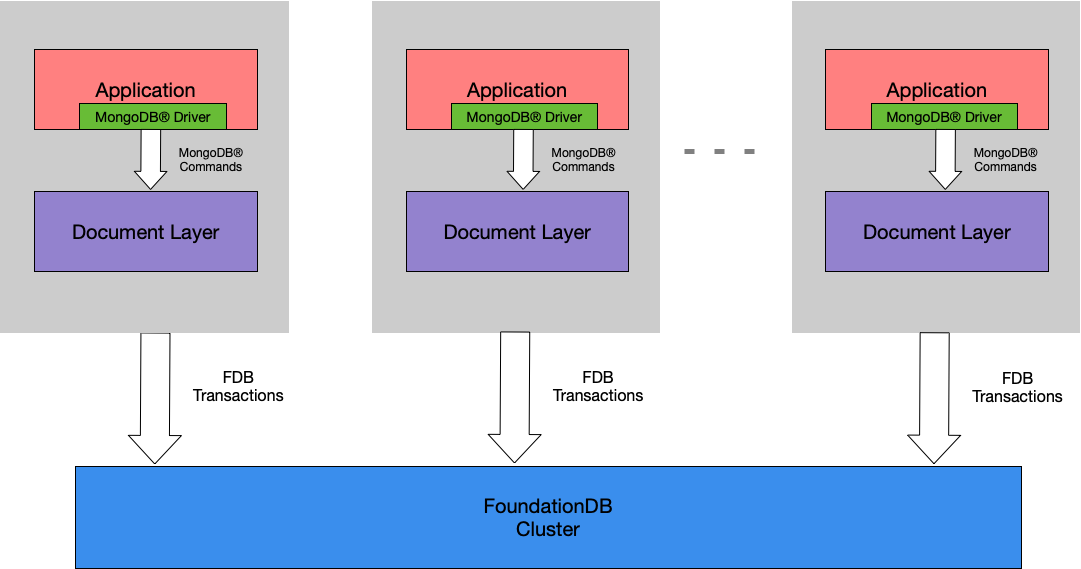
\includegraphics[width=0.6\textwidth]{img/1-Introduction/sidecar-arch.png}
\end{center}

\end{frame}

%------------------------------------------------


\begin{frame}
	\frametitle{Layer strategy}

FoundationBD is leaving the rest to additionals “layers”.

\vspace{0.5cm}
Examples:
\begin{itemize}
    \item \textbf{FoundationDB Record Layer}: Java Api that adds back much of what users expect from a simple relational database 
    \item CouchDB 4.0: adopt FoundationDB in 2019 as storage and replication engine.
\end{itemize}
\end{frame}
%------------------------------------------------

%%% ARCHITECTURE %%%

%------------------------------------------------

\begin{frame}
	\frametitle{Optimistic concurrency control P2}
While running, transactions use data resources \textbf{without acquiring locks on those resources}. Before committing, each transaction verifies that no other transaction has modified the data it has read. 
\vspace{0.2cm}

\begin{center}
    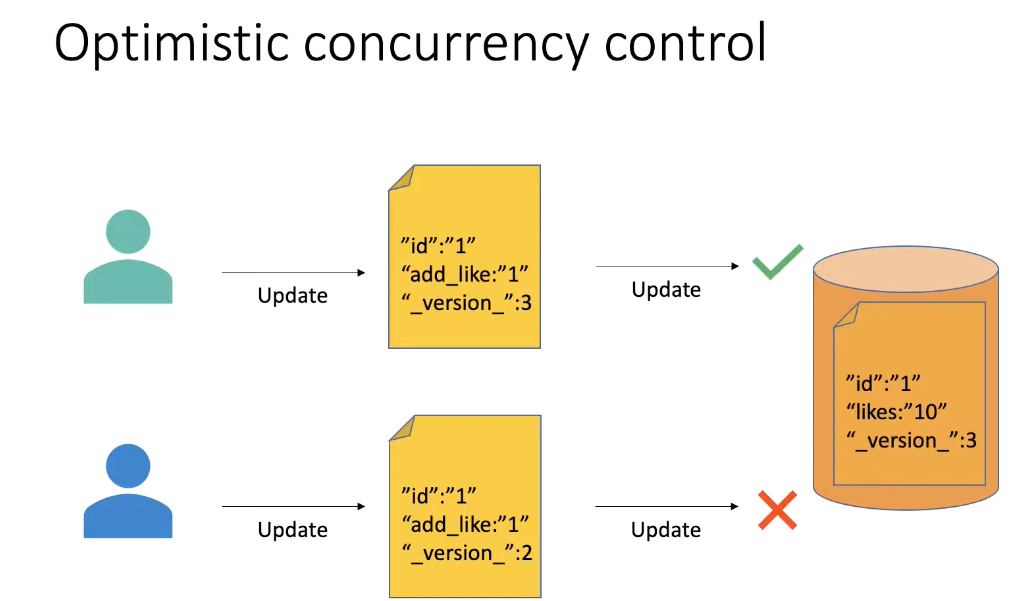
\includegraphics[width=0.5\textwidth]{img/2-Architecture/Optimistic Concurrency Control.png}
\end{center}

If the check (Resolvers) reveals conflicting modifications, the committing transaction rolls back and can be restarted.


\end{frame}

\begin{frame}
	\frametitle{Control plane P1}

The control plane is responsible for persisting critical metadata of the cluster for high availability.
\textbf{Cluster Controller} monitors all servers in the cluster and recruits 3 processes:
\begin{itemize}
    \item Sequencer (Data Plane)
    \item Data Distributor
    \item Ratekeeper
\end{itemize}

Coordinators form a Paxos group (consensus protocol) and elect the Cluster Controller.
\end{frame}

%------------------------------------------------


\begin{frame}
    \frametitle{Control plane P2}
    \begin{columns}
        \begin{column}{0.5\textwidth}
        \begin{itemize}
        \item \textbf{Data Distributor} is responsible for monitoring failures and balancing data among Storage Servers.
        \item \textbf{Ratekeeper} provides overload protection for the cluster.
        \end{itemize}
        
        \end{column}
        \begin{column}{0.5\textwidth}
            \centering
            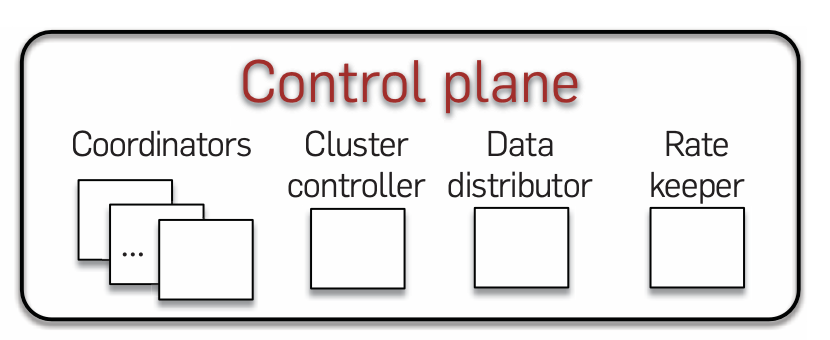
\includegraphics[width=\textwidth]{img/2-Architecture/Control plane.png}
        \end{column}
    \end{columns}
\end{frame}

%------------------------------------------------

\begin{frame}
	\frametitle{Data plane: Transaction system (TS) P2}

FoundationDB uses \textbf{multiversion concurrency control} to provide transactionally isolated reads without locking data or blocking writes.
\vspace{0.5cm}

\textbf{Optimistic concurrency control} ensures that deadlocks are impossible and that slow or failing clients cannot interfere with the operation of the database.
	
\end{frame}

%------------------------------------------------

\begin{frame}
	\frametitle{Scaling}
Scaling is just adding processes for each role. \\

\begin{itemize}
\item Clients read from sharded Storage Servers, so reads scale
linearly with the number of Storage Servers. 
\end{itemize}

\vspace{0.5cm}
Coordinators and control plane's singleton processes like \textbf{Cluster Controller} and \textbf{Sequencer} only perform limited metadata operations.
	
\end{frame}

% ------------------------------------------------

\begin{frame}
	\frametitle{After detecting a failure}
    \begin{itemize}
        \item The recovery process starts by
        detecting a failure and recruiting a new transaction system
        \item CC (Cluster Controller) reads the previous TS configuration from Coordinators and locks this information
        to prevent another concurrent recovery
        \item CC recovers previous TS system states, including information about older Log Servers
        \item CC recruits a new set of Sequencer, Proxies, Resolvers,
        and Log Servers
        \item need to ensure all transactions in the LS are durable and retrievable by Storage Servers for recovery

    \end{itemize}

\end{frame}

\begin{frame}
	\frametitle{Replication: Metadata, Log, Storage}
    \begin{itemize}
      \item System metadata of the control plane is stored on Coordinators using \textbf{Disk Paxos} (consensus protocol used for reliable data replication across multiple nodes optimized for disk storage)
      \item When a Proxy writes logs to Log Servers, each sharded log record is synchronously replicated on \textbf{multiple Log Servers}.
      \item Every shard (key range) is asynchronously replicated with multiple Storage Servers, forming a "\textbf{team}".

\end{itemize}
\end{frame}

%% TESTING %%

\begin{frame}
    \frametitle{Fault Injection}
    \begin{itemize}
        \item Simulation injects various faults such as machine failures, network partitions, and disk behavior.
        \item FDB cooperates with the simulation to make rare states and events more common through "\textbf{buggification}"
        \item Maximizes simulation diversity by randomizing cluster size, workloads, fault injection parameters.
    \end{itemize}
\end{frame} 